\chapter{プログラムと評価\hspace{-3mm}}

\section{プログラミング言語とは}

プログラミング言語とはプログラムを書くための言語です。プログラミング言
語の処理系とは、与えられたプログラムを計算するもので、コンパイラと実行
系の組み合わせで計算したり、インタープリタで計算したりします。本書では
プログラムを逐次解釈
し実行していくインタープリタを作って行きます。これは、与えら
れたプログラムの動作を規定するものですので、見方を変えれば、処理系であ
るインタープリタによりプログラミング言語を定義しているとも言えます
\footnote{これをプログラミング言語を操作的意味論(operetional semantics)で定義すると言います。}。

次にプログラムとは何か、という観点で上の文章を言い換えてみます。プログラム
は計算するための手順をしるしたものと言われていますが、本文書ではこれと
は異なる方法で定義します。すなわち、プログラムが与えられたをとき、
それをどう実行するかを定義します。
今回は、自然言語で書かれた仕様書ではなく、Rubyのプログラムによって、何をプログ
ラムとして受け入れ、それがどう実行されるのかを定めます。これにより、自
然言語に含まれるあいまいさがなく、プログラムとは何かを定めることができます。

はじめから全てのプログラムを対象にすると理解が難しいので、簡単なプログ
ラムの例を示しながら、それが動くように少しずつ機能を追加していきます。

“プログラミング言語の処理系”なんて難しく考えないでください。要は、文字列を
読み込んで、それを計算するプログラムです。電卓に毛が生えたものと思えば
気も楽になりませんか。最初はまさに電卓の例から考えてみます。

\section{はじめてのプログラムの評価}

最初のプログラムとして次のプログラムを考えます。

\begin{lstlisting}
[:+, 1, 2]
\end{lstlisting}

今までのプログラムと全く異なる記述方法に戸惑うことでしょう。当然です。これは著者が勝手に考えた$\mu$SchemeR(名前も勝手に考えました)というプログラミング言語だからです。気にくわない書き方だと思いますが、この文書を読み終わるころには、自分の好きな書き方へ直す力が身についていると思いますので少しお付き合い下さい。

ただ少し想像力を働かせれば、1と2を足し合わせるプログラムなのだと想像できるのではないでしょうか。そのとおり、正解です。では、“このプログラムを与えられた時にこの結果を求める処理を考えて下さい”と言われたとき、どう答えるでしょうか。“1と2を足し合わせた結果を求める”もしくは“{\tt :+}が先頭にあった時、続く2つの引数の値を足し合わせる”とも言えるでしょう。

では、次のプログラムの結果を求める処理はどうでしょう。

\begin{lstlisting}
[:+, [:+, 1, 2], 3]
\end{lstlisting}

“まず{\tt [:+, 1, 2]}を計算してその結果と3とを足し合わせる”と言えるでしょう。ここで前回の説明に“計算して”という言葉が加わったことに気づいたでしょうか。すなわち、上2つのプログラムの計算結果を求める処理を考えたとき、その処理は{\tt :+}に続く引数を“計算”した後に足し合わせる必要があるのです。通常、我々はこの計算のことを“評価(evaluation)”と言います。したがって、“{\tt :+}が先頭にあった時、続く2つの引数を評価して、その値を足し合わせる”が求める処理です。

% \begin{boxnote}
% {\bf コラム: $\mu$SchemeRのシンタックス} \\

\begin{breakitembox}[l]{\bf コラム: $\mu$SchemeRのシンタックス} 
今回作成するプログラミング言語$\mu$SchemeRでは、{\tt [:+, 1, 2]}などのように
最初に関数を、その後引数を記述します。なぜ、このようなスタイルなのでしょう。他言語のように{\tt x + y * z}と書かかれたものを計算するためには{\tt (x + y) * z}なのか{\tt x + (y * z)}なのかを演算子の優先度を考慮して決める必要があります。さらに言えば、後に出てくるif文も{\tt [:if, :true,  1, 0]}などのように必ず{\tt [}の後に{\tt :if}のようなキーワードが出てくるので、この文字列を見れば通常の関数適用なのか、特殊な構文なのかを簡単に解釈できます。一方で、{\tt if (true) then 1 else 2;}や{\tt x = y + 1;}などのように色々な形の構文を許すとそれがどのような構文なのかを解釈するために多くの計算(字句解析/構文解析)が必要になってきます。計算機がこの処理をせずに人間がこの作業をすることで、計算機側は簡単な処理でそれを解釈できるようになっていると言うわけです\footnotemark[2]。
また、要素は“{\tt ,}”で区切りそれらを“{\tt [}”と“{\tt ]}”で囲みリストを表します。この形式は、Rubyで配列としてそのまま扱えるため、計算機側で余計な処理を考えなくて良くなります。また、記号である{\tt +}や変数である{\tt x}や予約語{\tt if}などは、単語のはじめに{\tt :}をつけてそれぞれ{\tt :+}、{\tt :x}、{\tt :if}と記します。この表記法もRubyでそのままシンボル\footnotemark[3]として扱えるために導入しています。
% \end{boxnote}
\end{breakitembox}
\footnotetext[2]{このことは計算機がすべきことを人間が苦労を強いられているという単純な話ではありません。なぜならプログラミング言語の仕様が単純になるため、結果的に言語仕様を学習する労力が削減されるためです。言語習得の容易さとプログラムの書きやすさのバランスが求められるのかもしれません。}
\footnotetext[3]{Rubyでは{\tt :}に文字列を続けることで、それを定数のように扱えるシンボルという機能が存在します。シンボルを使わない場合、{\tt x}を評価するとRuby上の変数として評価されるため、{\tt x}がRubyで定義されていない場合エラーになるため扱いが面倒となります。}

\setcounter{footnote}{3}

それでは、このプログラムの結果を求める処理をRubyで記述してみましょう。

{\tt \_eval}\footnote{{\tt eval}としないで{\tt \_eval}としているのは、Rubyの組み込み関数として{\tt eval}が定義されているためです。気になる人は、Rubyの{\tt module}機能を使って名前空間を分け、{\tt \_eval}を{\tt eval}として定義しなおして下さい。またその際は、p. \pageref{fun:parse}の{\tt parse}で使われる{\tt eval}は{\tt Kernel::eval}に置き換えて下さい。}は、与えられた式{\tt exp}を評価し、その結果を返します。

式がリストであった場合、最初の要素を関数として、残りを引数として、それぞれを評価してその値を求めます。求めた関数に求めた引数の値を適用(apply)してその結果を{\tt \_eval}の結果とします\footnote{Rubyでは、関数の最後に評価した式の値が関数の返り値になります。一般的に関数型言語では{\tt return} {\it {\tt <}値{\tt >}}と書かずに、このような書き方をします。本書では、関数型言語の考え方に近づくようにこの記述を利用していきます。}。一方、リストでない場合、数字であれば即値として扱い数字そのものを返します。例えば{\tt 2}は2を返します。そうでなければ、組み込み関数とみなし、それに関連付けられた(Ruby上での)関数を返します。

\begin{lstlisting}
def _eval(exp)
  if not list?(exp) 
    if immediate_val?(exp)
      exp
    else 
      lookup_primitive_fun(exp)
    end
  else
    fun = _eval(car(exp))
    args = eval_list(cdr(exp))
    apply(fun, args)
  end
end
\end{lstlisting}

% \begin{boxnote}
% {\bf コラム: プログラムコードと値の区別} \\
\begin{breakitembox}[l]{\bf コラム: プログラムコードと値の区別} 
“{\tt 2}は2を返します”という文章で数字のフォントが違っていることに気づきましたか? {\tt 2}は(現在考えている$\mu$SchemeR)プログラムの、2は(Ruby上での)数値の2を表します。こう記載することによって、プログラムとその評価された値とを区別します。図\ref{fig:uschemer_ruby}を確認してください。
% \end{boxnote}
\end{breakitembox}

以降、上のRubyプログラムで呼ばれている関数を説明していきます。

リストかどうかは配列のインスタンスかどうかで判断しています。

\begin{lstlisting}
def list?(exp)
  exp.is_a?(Array)
end
\end{lstlisting}

組み込み関数は、関数名をキーに、関数本体をその値としたハッシュで保有しま
す。関連付けられている関数はRuby上での関数です。組み込み関数の評価は、
関数名に関連付けられた関数を値として返します。

\begin{lstlisting}
def lookup_primitive_fun(exp)
  $primitive_fun_env[exp]
end

$primitive_fun_env = {
  :+ => [:prim, lambda{|x, y| x + y}],
  :- => [:prim, lambda{|x, y| x - y}],
  :* => [:prim, lambda{|x, y| x * y}], 
}
\end{lstlisting}

{\tt car}はリストの先頭の要素を、{\tt cdr}は先頭の要素以降のリストを取得する関数です。この名前は奇妙\footnote{carはContents of the Address part of Register、cdrはContents of the Decrement part of Register、後で出てくるconsはCONStructから来ています。これらはLispが開発されたIBMの計算機の機械語に由来しています。} ですが、Schemeで使われている名前ですので我慢してください。そのうち慣れてくるでしょう。

\begin{lstlisting}
def car(list)
  list[0]
end

def cdr(list)
  list[1..-1]
end
\end{lstlisting}

引数を評価する{\tt eval\_list}は、リストの要素それぞれを評価したものをリストにしたものです。

\begin{lstlisting}
def eval_list(exp)
  exp.map{|e| _eval(e)}
end    
\end{lstlisting}

そのままの値を返す即値として数字を定義しています。

\begin{lstlisting}
def immediate_val?(exp)
  num?(exp) 
end

def num?(exp)
  exp.is_a?(Numeric)
end
\end{lstlisting}

関数適用は、引数の評価値(Ruby上の値になります)を(Ruby上の)関数へ適用しています。
{\tt fun\_val.call(*args)}は、{\tt fun\_val}というRuby上の関数を引数{\tt args}で呼び出します。{\tt *}は、可変長引数に対応しており、{\tt args}が{\tt [1, 2]}の場合{\tt fun\_val.call(1, 2)}と展開され、{\tt args}が{\tt [1, 2, 3]}の場合{\tt fun\_val.call(1, 2, 3)}と展開されます。

\begin{lstlisting}
def apply(fun, args)
  apply_primitive_fun(fun, args)
end

def apply_primitive_fun(fun, args)
  fun_val = fun[1]
  fun_val.call(*args)
end

def primitive_fun?(exp)
  exp[0] == :prim
end
\end{lstlisting}

実際に、{\tt [:+, 1, 2]}を評価するときの動きを図\ref{fig:uschemer_ruby}を見ながら追ってみましょう。与えるプログラムはリストですので、まず先頭の要素{\tt :+}を評価し、$lambda\{|x, y| x + y\}$を値として得ます。これは、二つの引数を足す(Ruby上の)関数です。次に{\tt 1}, {\tt 2}を評価し、それぞれ(Ruby上での)1, 2を得ます。これを(Ruby上で)適用することで、3を得ます。この値はputsを使って、Ruby上のプログラムで表示することができます\footnote{今回作成している$\mu$SchemeR上でも、表示出来まるようにしますが、後のお楽しみとします。}。

\begin{figure}[htbp]
\begin{center}
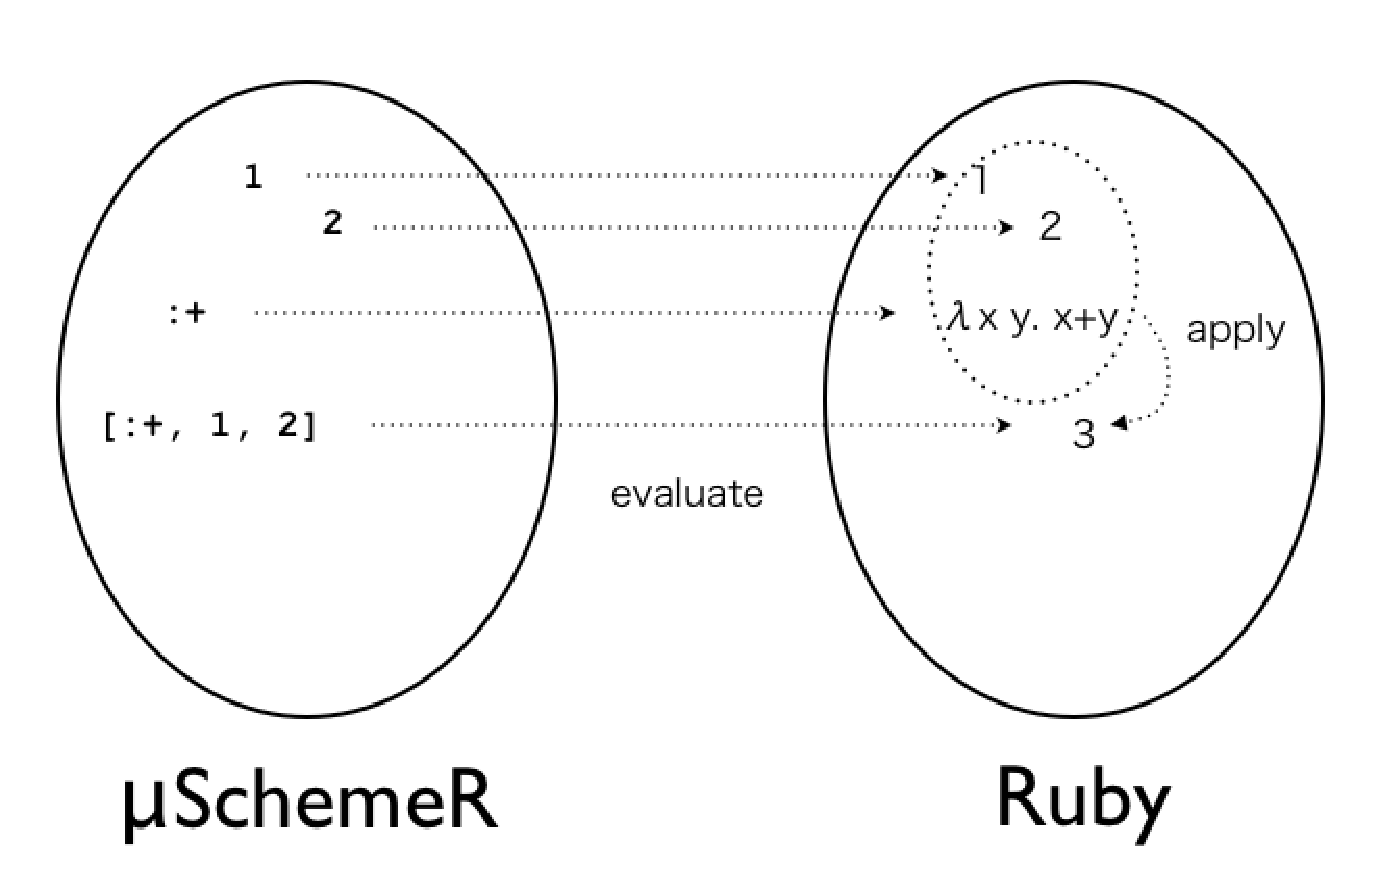
\includegraphics[width=80mm]{images/uschemer_ruby.eps}
\end{center}
\caption{プログラミング言語の世界$\mu$SchemeRと評価値の世界Rubyとの関係}
\label{fig:uschemer_ruby}
\end{figure}


\begin{lstlisting}
puts _eval([:+, 1, 2])
\end{lstlisting}

を実行して3が表示されましたか。おめでとうございます。おそらく、あなたははじめてプログラミング言語のインタープリタを作ったのではないでしょうか。足し算程度しか出来ないプログラミング言語なので実感は無いかもしれませんが、正真正銘のプログラミング言語の処理系です。

{\tt [:+, [:+, 1, 2], 3]}が評価される流れも自分で追ってみて下さい。{\tt \_eval}が再帰的に呼ばれている点が役立っていることに気づけましたか。

\section{まとめ}

この章では次のことを学びました。

\begin{itemize}
\item 簡単なプログラムの計算方法(また、我々はこの計算を“評価”と呼びました)
\item 関数適用の評価方法、すなわち、関数と引数を評価して、得られた関数の評価値に引数の評価値を関数適用するということ
\item プログラムが評価されると(プログラムの実行結果はRubyという)他の世界の値として得られること
\end{itemize}

普段何気なく書いている{\tt x = y;}というプログラムは、実際は右辺をまず評価してその値を左辺の変数のアドレスに格納する、ということを行っています。漠然とは理解していたと思いますが、実際は本章で学んだ評価という考え方などに基づいてプログラムは実行されています。その内部を少し垣間見ることが出来たのではないでしょうか。
